\lecture{Metodologias de Desenvolvimento de Software}{methods}

\lecturetitle{\course}{\insertlecture}

\frame{\maketitle}

\section{Princípios da Engenharia de Software}

\begin{frame}{Princípios de desenvolvimento de software/sistemas}

  \begin{description}[<+-| alert@+>]
  \item[Formalização:] aplicação de métodos formais para aumento da
    confiabilidade;
  \item[Abstração:] representação do mundo real com nível de
    detalhamento adequado para eliminação da complexidade;
  \item[Decomposição:] divisão em partes menores para redução 
    da complexidade;
  \item[Generalização:] descoberta ou adoção de princípios
    fundamentais que permitem reutilização;
  \item[Flexibilização:] adaptação è evolução, extensão e
    aperfeiçoamento.
  \end{description}
  
\end{frame}

\section{Ciclo de vida do software}
  
\begin{frame}{Ciclo de vida do software}

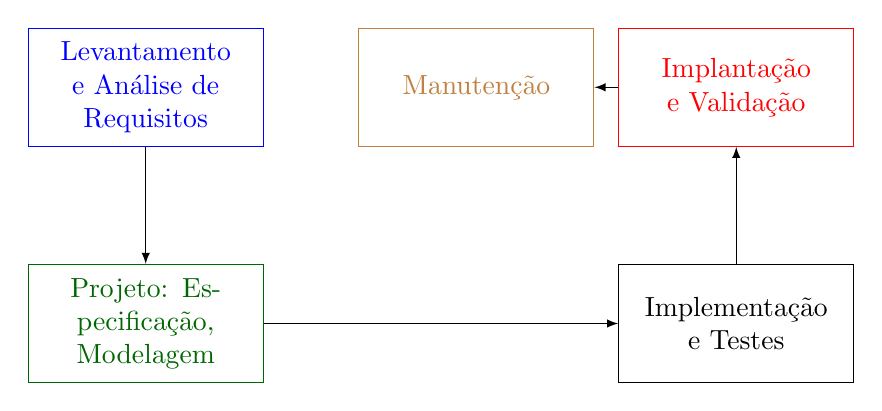
\begin{tikzpicture}
  [cycle/.style={text centered,text width=2.75cm,minimum width=2cm,
    minimum height=1.5cm,draw},every path/.style={->,>=latex,draw}]
  \def\D{2cm}

  \node<1->[cycle,blue] (spec) {Levantamento e Análise de Requisitos};
  \node<2->[cycle,green!40!black] (proj) [below of=spec,yshift=-\D] {Projeto: Especificação, Modelagem};
  \node<3->[cycle] (dev) [right of=proj,xshift=3.25*\D] {Implementação e Testes};
  \node<4->[cycle,red] (deploy) [above of=dev,yshift=\D] {Implantação e Validação};
  \node<5->[cycle,brown] (maintain) [left of=deploy,xshift=-1.15*\D] {Manutenção};
  
  \path<2-> (spec) -- (proj);
  \path<3-> (proj) -- (dev);
  \path<4-> (dev) -- (deploy);
  \path<5-> (deploy) -- (maintain);
\end{tikzpicture}

%%
% Local variables:
% mode: latex
% End:
%%

\end{frame}


\begin{frame}{Desenvolvimento em Cascata}

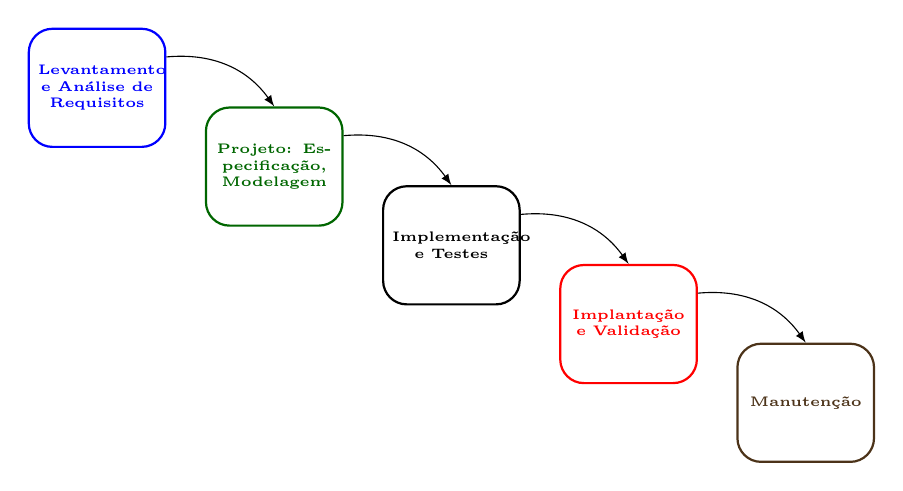
\begin{tikzpicture}
  [font={\tiny\bf},node distance=2.25cm,every path/.style={->,>=latex,draw},
  cycle/.style={thick,rounded corners=3mm,text centered,text width=1.5cm,minimum width=1cm, minimum
    height=1.5cm,draw},
  dev/.style={cycle},
  deploy/.style={cycle,red},
  maintain/.style={cycle,brown!40!black}]

  \node<1->[cycle,blue] (requirements) {Levantamento e Análise de Requisitos};
  \node<2->[cycle,green!40!black] (proj) [right of=requirements,yshift=-1cm] {Projeto: Especificação, Modelagem};
  \node<3->[dev] (dev) [right of=proj,yshift=-1cm] {Implementação e Testes};
  \node<4->[deploy] (deploy) [right of=dev,yshift=-1cm] {Implantação e Validação};
  \node<5->[maintain] (maintain) [right of=deploy,yshift=-1cm] {Manutenção};
  
  \path<2-> (requirements) edge [bend left] (proj.north);
  \path<3-> (proj) edge [bend left]  (dev.north);
  \path<4-> (dev) edge [bend left]  (deploy.north);
  \path<5-> (deploy) edge [bend left]  (maintain.north);
\end{tikzpicture}
  

\end{frame}

\begin{frame}{Método Evolutivo}
  \begin{center}
  \begin{tikzpicture}
    [font=\scriptsize,phase/.style={minimum height=1cm,draw},
    protophase/.style={minimum width=3cm,ellipse,draw},
    version/.style={white,fill=black,circle,draw},
    every path/.style={->,>=latex,draw}]

    \node[phase,tape,thick] (requirements) {Requisitos};
    \node[thick,minimum height=5cm,minimum width=3.2cm,draw] (prototype) [right of=requirements,xshift=2cm] {};
    \node[above] at (prototype.north) {Prototipação};
    \node[fill=yellow,protophase] (dev) [right of=requirements,xshift=2cm,yshift=1cm]
    {Implementação};
    \node[fill=gray,protophase] (eval) [right of=requirements,xshift=2cm,yshift=-1cm]  {Validação};
    
    \node[version] (v0) [right of=prototype,xshift=2cm,yshift=2.5cm] {Versão
      0};
    \node[version] (v1) [right of=prototype,xshift=2cm]
    {Versão 1};
    \node[]  [right of=prototype,xshift=2cm,yshift=-1.25cm] {$\vdots$};
    \node[version] (vN) [right of=prototype,xshift=2cm,yshift=-2.5cm] {Versão N};

    \path (requirements) -> (prototype);
    \path (dev.south west) -> (eval.north west);
    \path (eval.north east) -> (dev.south east);
    \path (prototype.north east) -> (v0);
    \path (prototype.east) -> (v1);
    \path (prototype.south east) -> (vN);
  \end{tikzpicture}
\end{center}

\end{frame}


\begin{frame}{Método Evolutivo}

\begin{block}{Vantagens}
  \begin{itemize}[<+-| alert@+>]\setbeamercovered{transparent}
  \item Verificação antecipada de possíveis problemas durante a
    implementação: linguagem de programação, algoritmo, performance.
  \item Maior interação com o cliente, permitindo esclarecer dúvidas
    sobre requisitos que não estejam bem definidos.
  \end{itemize}
\end{block}  

\end{frame}

\begin{frame}{Método Evolutivo}

\begin{block}{Desvantagens}
  \begin{itemize}[<+-| alert@+>]\setbeamercovered{transparent}

    \item Não é dada atenção à documentação, pois cada protótipo é
      visto como provisório.

  \item Pode causar inconsistências na estrutura do projeto.
    \note{Envolve o mito de que alterações são fáceis}

    \item Dá a impressão ao cliente, em algumas versões, de que o
      projeto está quase pronto.
      \note{O cliente irá pressionar para usá-lo, achando que somente
        algumas alterações são necessárias}

    \item O desenvolvedor pode fazer escolhas inapropriadas para
      adiantar um protótipo, prejudicando as versões seguintes.
  \end{itemize}
\end{block}

\end{frame}


\begin{frame}{Método Espiral}{Boehm}
  
  \begin{block}{Características}
    \begin{itemize}[<+-| alert@+>]\setbeamercovered{transparent}
    \item Incorpora características dos processos em cascata e
      evolutivo, com a adição da análise de risco.
      \note{Dá atenção especial às partes críticas do projeto}
    \item Cada iteração da espiral se beneficia das lições da anterior.
    \item O protótipo está mais voltado para o projeto e não para o
      funcionamento do sistema.
      \note{Evita expectativas do cliente com relação ao programa.}
      \item Mais flexível que o cascata;
      \item O protótipo não é funcional, o que provoca riscos em caso
        de pressão para produzir algo ou corte de gastos;
    \end{itemize}
  \end{block}
\end{frame}


\begin{frame}{Método Espiral}

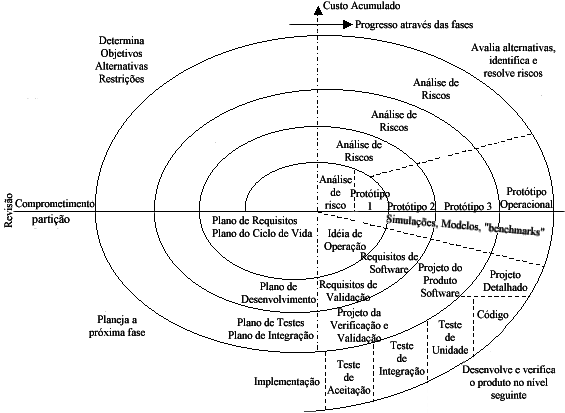
\includegraphics[scale=.4]{img/spiral.png}

\vfill
{\tiny Fonte: \href{http://www2.dem.inpe.br/ijar/CicoloVidaSoftPrado.html}{Engenharia de Software, Capítulo 2 - Ciclo de Vida do Software, Professor Prado.}}
\end{frame}


\lecture{Rational Unified Process (RUP)}{RUP}

\begin{frame}{\insertlecture}
  Processo baseado na UML ({\em Unified Modeling Language}) criado
  pela Rational Corp., adquirida pela IBM. O processo baseia-se nas
  fases conforme a figura a seguir:

  \begin{center}
    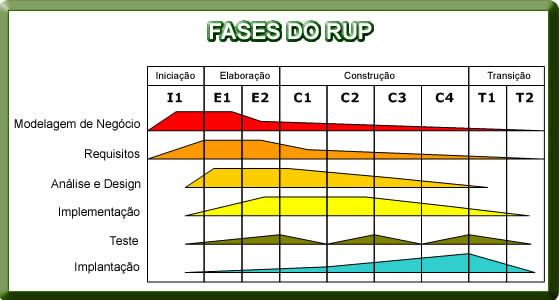
\includegraphics[scale=.6]{img/fasesRUP.png}\\
    {\tiny Fonte: \href{https://www.infoescola.com/engenharia-de-software/rup/}{RUP. Marina Martinez.}}
  \end{center}
\end{frame}

\begin{frame}{\insertlecture}{Fases}
  \begin{enumerate}[<+-| alert@+>]\setbeamercovered{transparent}
  \item {\bf Concepção/Iniciação}: define o escopo do projeto,
    cronograma e despesas. É usado para verificar o progresso.
  \item {\bf Elaboração}: trabalho com o cliente para identificar
    casos de uso, projeta a arquitetura de software, ajusta o plano de
    desenvolvimento e constrói um protótipo inicial.
  \item {\bf Construção}: codifica e testa o produto, resultando no
    primeiro lançamento de teste.
  \item {\bf Transição}: move o produto do ambiente de desenvolvimento
    para o ambiente de produção, onde inclui o teste de aceitação do
    cliente e o treinamento do usuário.
  \end{enumerate}
\end{frame}

\begin{frame}{\insertlecture}{\em Workflows}
  \begin{enumerate}[<+-| alert@+>]\setbeamercovered{transparent}
  \item Modelagem de negócio;
  \item Requisitos;
  \item Análise e especificação/design;
  \item Implementação;
  \item Teste;
  \item Implantação.
  \end{enumerate}
\end{frame}

\begin{frame}{\insertlecture}{Considerações}
  \begin{itemize}
  \item Diferente do Cascata, cada fase do RUP envolve iteração. Por
    exemplo, a concepção pode ter uma iteração, a elaboração duas, a
    construção quatro e a transição duas. Como o Espiral, o RUP pode
    iterar através das quatro fases repetidamente.
  \end{itemize}  
\end{frame}

\begin{frame}{Abordagem de Planejar-Documentar}
  \begin{itemize}[<+-| alert@+>]\setbeamercovered{transparent}
  \item O métodos e processos vistos exigem uma abordagem
    que envolve Planejamento e documentação, por isso, são considerados
    mais pesados do que as abordagens Ágeis.
  \item Alguns programadores consideram estas metodologias tediosas 
    para o desenvolvimento de software.
  \end{itemize}
\end{frame}

% \begin{frame}{Métodos ágeis}
  
%   \begin{block}{Características}
%     \begin{itemize}[<+->]
%     \item Código como principal medida de progresso;
%     \item Colaboração entre desenvolvedores e clientes que participam
%       mais ativamente das fases de desenvolvimento;
%     \item Comunicação frequente;
%     \item Simplificação da documentação;
%     \item Testes como guias para o desenvolvimento;
%     \item Desenvolvimento em pequenos incrementos com integração contínua;
%     \item Práticas como programação em grupos de duas pessoas.
%       \note{Para aumentar o número de pessoas pensando sobre as
%         decisões técnicas e capturar erros mais facilmente.}
%     \end{itemize}
%   \end{block}
% \end{frame}


\begin{frame}{Referência}
  \begin{itemize}
  \item {\color{blue}''Engineering Software as a Service: An Agile Approach Using
    Cloud Computing.''} Armando Fox,‎ David Patterson. Strawberry Canyon
    LLC, 2014.
  \end{itemize}  
\end{frame}